\documentclass{article}

\usepackage{graphicx}
\usepackage{tikz}
\usepackage{tikzsymbols}
\usetikzlibrary{calc,patterns,shapes.geometric}
\pagestyle{empty}
\usepackage[margin=0pt]{geometry}
\geometry{papersize={14in,12in}}

\def\centerarc[#1](#2)(#3:#4:#5){\draw[#1] ($(#2)+({#5*cos(#3)},{#5*sin(#3)})$) arc (#3:#4:#5);}

\begin{document}
	\begin{figure}
		\centering
		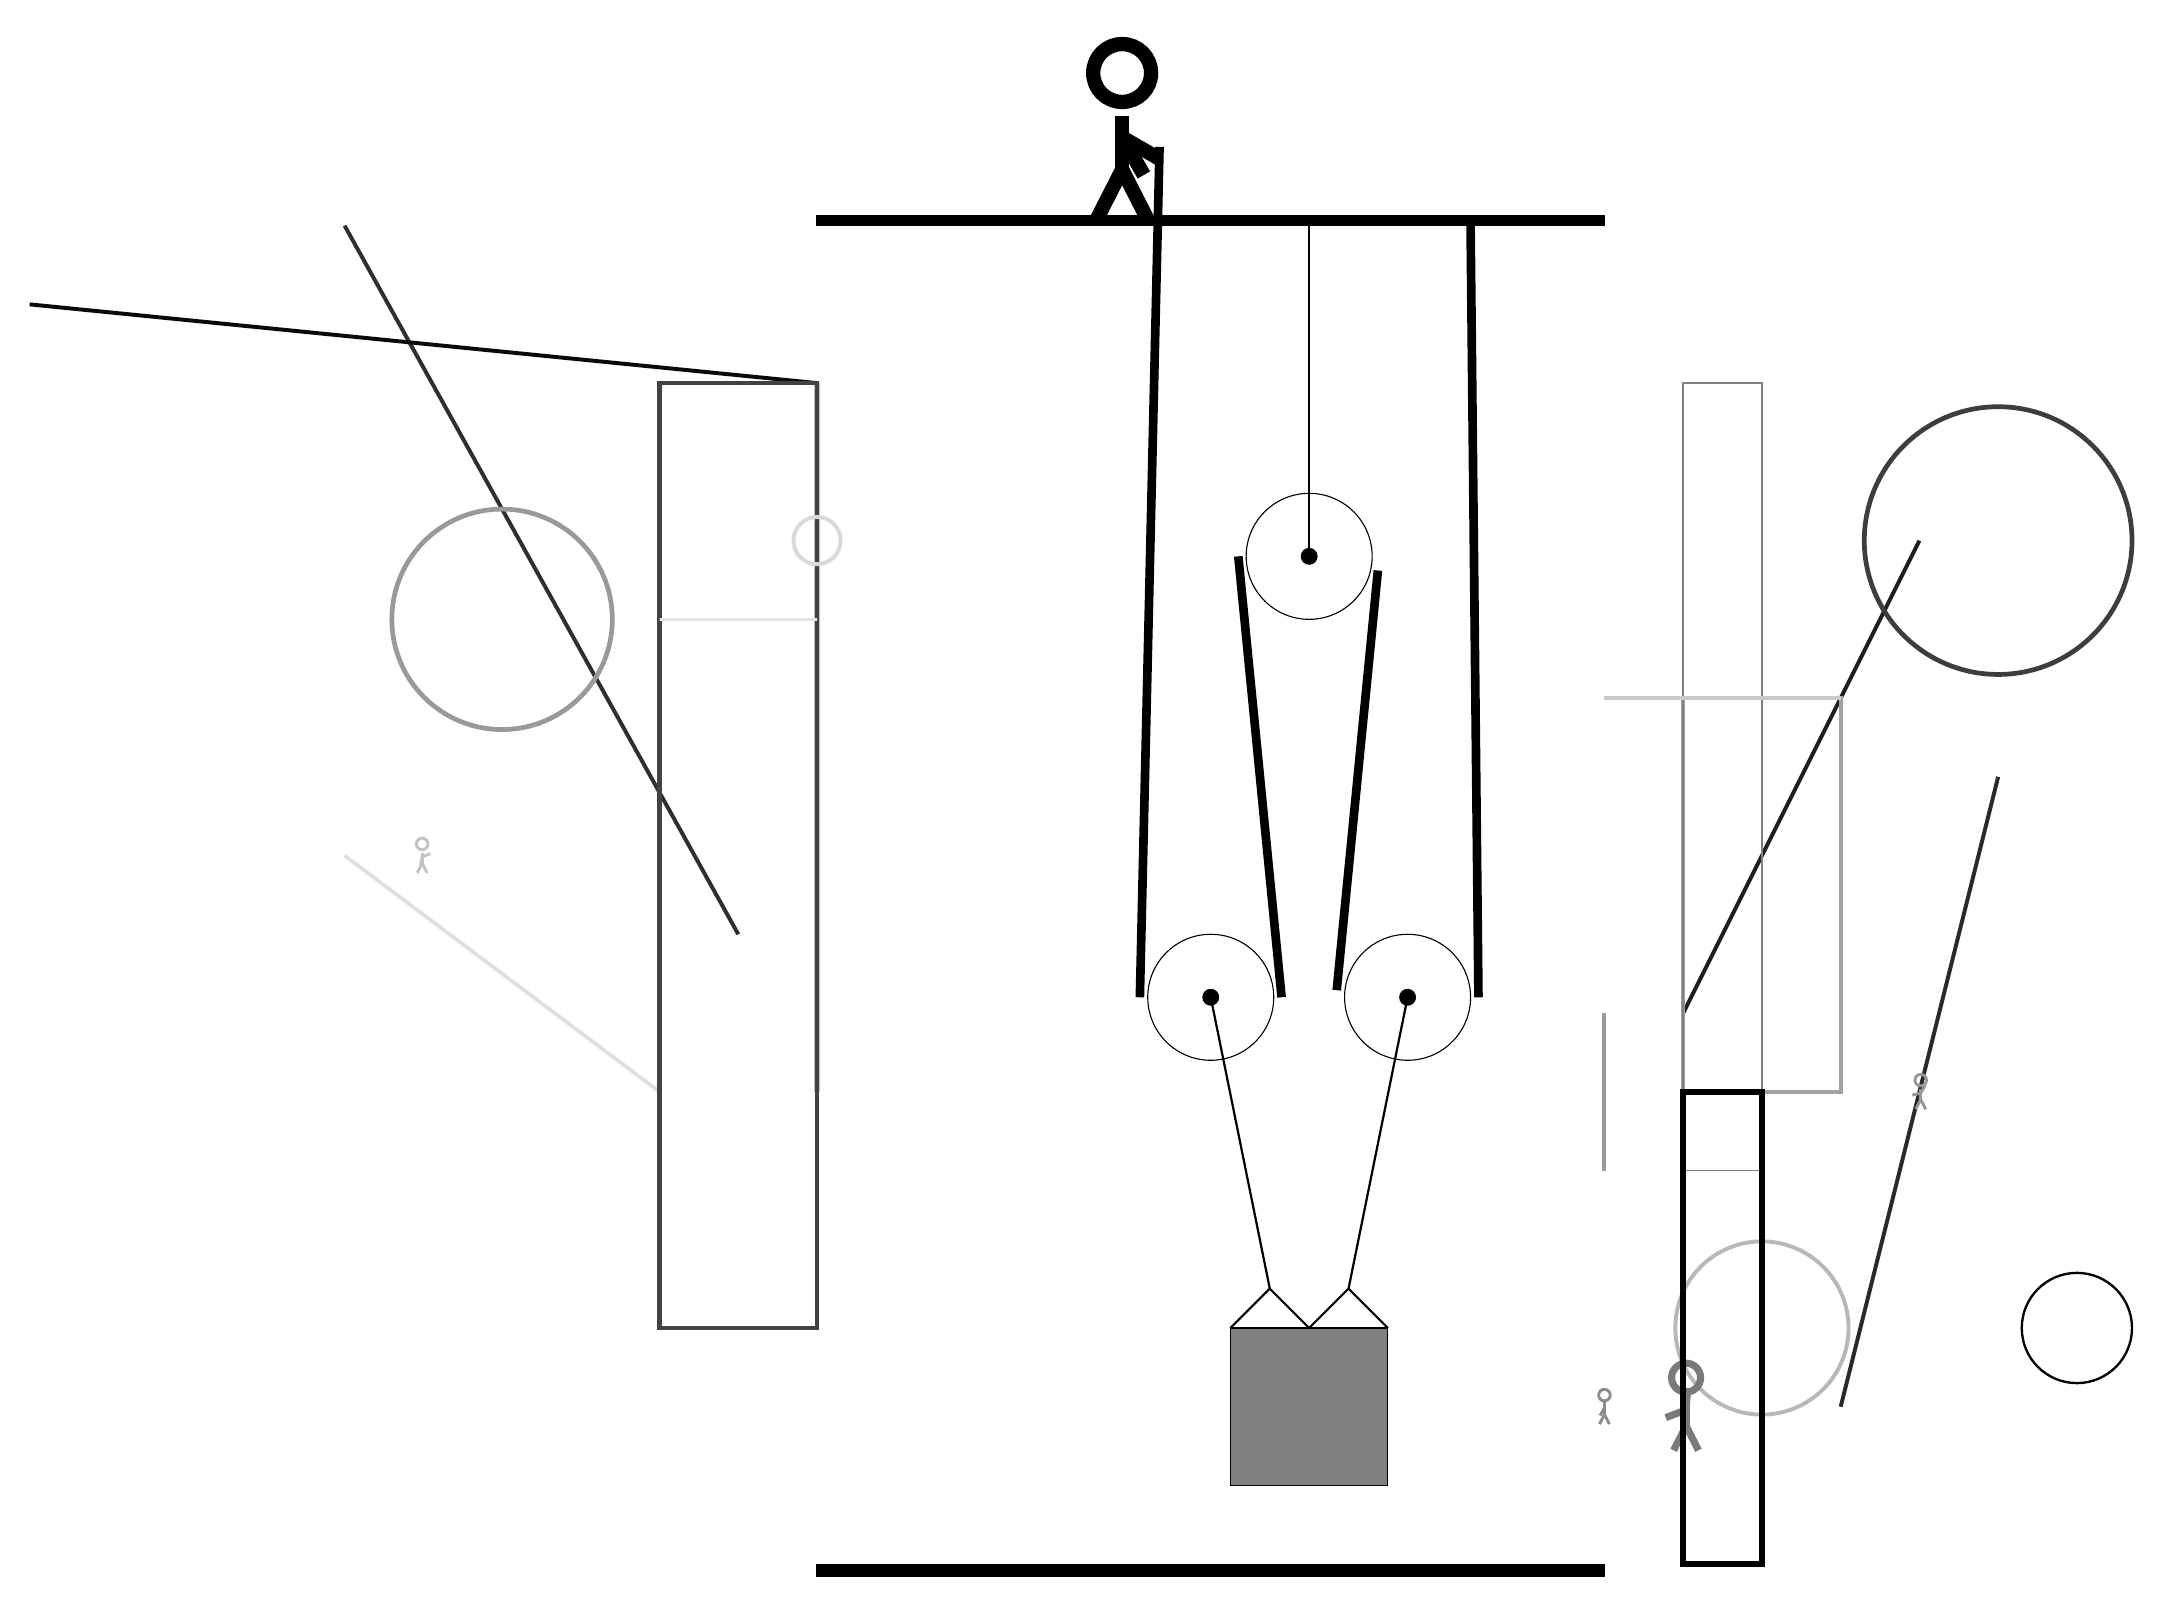
\begin{tikzpicture}
			%%%%% START %%%%%
			
			\draw[fill=black] (-4, 14) rectangle (6, 14.125);
			
			\draw (1, 4.2) circle (0.8);
			\draw[fill=black] (1, 4.2) circle (0.1);
			
			\draw (2.25, 9.8) circle (0.8);
			\draw[fill=black] (2.25, 9.8) circle (0.1);
			\draw[thick] (2.25, 9.8) -- (2.25, 14);
			
			\node[line width=0.2mm, color=black!45] at (6, -1) {\Strichmaxerl[2][60][89]};
			
			\draw[line width=0.5mm, color=black!88](7, 4) -- (10, 10);
			\draw[line width=0.5mm, color=black!40](6, 4) -- (6, 2);
			\draw [line width=0.3mm, color=black!99](12, 0) circle (0.7);
			
			\draw[line width=0.5mm, color=black!12](-6, 3) -- (-10, 6);
			
			\draw[line width=0.5mm, color=black!37] (7, 3) rectangle (9, 8);
			
			\draw[line width=0.5mm, color=black!82](-5, 5) -- (-10, 14);
			\node[line width=0.5mm, color=black!24] at (-9, 6) {\Strichmaxerl[2][79][20]};
			\draw[line width=0.7mm, color=black!24] (-4, 12) rectangle (-4, 3);
			\draw[line width=0.5mm, color=black!96](-4, 12) -- (-14, 13);
			
			\draw [line width=0.6mm, color=black!76](11, 10) circle (1.7);
			\draw[line width=0.6mm, color=black!74] (-4, 0) rectangle (-6, 12);
			\draw[line width=0.5mm, color=black!84](9, -1) -- (11, 7);
			
			\draw[line width=0.2mm, color=black!50] (7, 12) rectangle (8, 2);
			\draw [line width=0.6mm, color=black!40](-8, 9) circle (1.4);
			\draw [line width=0.5mm, color=black!28](8, 0) circle (1.1);
			
			\node[line width=0.6mm, color=black!52] at (7, -1) {\Strichmaxerl[5][21][86]};
			\draw [line width=0.5mm, color=black!15](-4, 10) circle (0.3);
			\draw[line width=0.5mm, color=black!21](6, 8) -- (9, 8);
			\node[line width=0.4mm, color=black!41] at (10, 3) {\Strichmaxerl[2][14][60]};
			\draw[line width=0.3mm, color=black!10] (-4, 9) rectangle (-6, 9);
			
			\draw[line width=0.7mm, color=black!100] (7, 3) rectangle (8, -3);
			\draw [line width=0.5mm, color=black!42](11, 5) circle (0.0);
			
			\draw (3.5, 4.2) circle (0.8);
			\draw[fill=black] (3.5, 4.2) circle (0.1);
			
			\draw[thick] (3.5, 4.2) -- (2.75, 0.5);
			\draw[thick] (1, 4.2) -- (1.75, 0.5);
			\draw[thick]  (1.25, 0) -- (1.75, 0.5) -- (2.25, 0);
			\draw[thick]  (2.25, 0) -- (2.75, 0.5) -- (3.25, 0);
			\draw[fill=black!50] (1.25, 0) rectangle (3.25, -2);
			
			\draw[line width=1.1mm] (0.35, 15) --  (0.1, 4.2);
			\centerarc[line width=1.1mm](1, 4.2)(180:360:0.9);
			\draw[line width=1.1mm] (1.9, 4.2) -- (1.35, 9.8);
			\centerarc[line width=1.1mm](2.25, 9.8)(-20:180:0.9);
			\draw[line width=1.1mm](3.123, 9.62) -- (2.6, 4.29);
			\centerarc[line width=1.1mm](3.5, 4.2)(160:360:0.9);
			\draw[line width=1.1mm](4.4, 4.2) -- (4.3, 14);
			
			\node at (-0.07, 15.2) {\Strichmaxerl[10][120][-30]};
			
			\draw[fill=black] (-4, -3) rectangle (6, -3.15);
			
			%%%%% END %%%%%
		\end{tikzpicture}
	\end{figure}	
\end{document}